\documentclass[10pt]{article}
\usepackage{comment}
\usepackage{listings}
\usepackage{graphicx}
\usepackage{psfrag}
\usepackage{amssymb}
\usepackage{amsmath}
\usepackage{algorithm2e}
\usepackage{caption}
\usepackage{epstopdf}
\usepackage{url}
\usepackage{fullpage}

\usepackage{float}
\floatplacement{figure}{H}

%\usepackage{epsfig}
%\usepackage{subfigure}


\begin{comment}
\newtheorem{theorem}{Theorem}[section]
\newtheorem{proposition}[theorem]{Proposition}
\newtheorem{lemma}[theorem]{Lemma}
\newtheorem{corollary}[theorem]{Corollary}
\newtheorem{definition}[theorem]{Definition}
\end{comment}


\usepackage{enumerate}
\usepackage{float}
\usepackage{flafter}
\usepackage{psfrag}
\usepackage{overpic}
\usepackage{subfigure}
\usepackage{caption}
\usepackage{multirow}
\usepackage{array}

\usepackage{amsmath}

%\usepackage{graphicx}
%\usepackage{caption}
%\DeclareCaptionType{copyrightbox}
%\usepackage{subcaption}
%\usepackage[on]{auto-pst-pdf} % enable psfrag for pdflatex
%\usepackage{xcolor}


\usepackage{epsfig}



\usepackage{color}% Include colors for document elements (required for psfrag)

\newcommand{\psdir}{./sections}
\newcommand{\ldir}{./sections}
\newcommand{\fig}{./sections/fig}
\newcommand{\comm}[1]{}


\def\IL{{\it left}}
\def\IM{{\it middle}}
\def\IR{{\it right}}
\def\IB{{\it bottom}}
\def\IT{{\it top}}


\newcommand{\algref}[1]{Algorithm~\ref{#1}}
\newcommand{\defref}[1]{Definition~\ref{#1}}
\newcommand{\secref}[1]{Section~\ref{#1}}
\newcommand{\figref}[1]{Fig.~\ref{#1}}
\newcommand{\exref}[1]{Ex.~#1}
\newcommand{\tabref}[1]{Table~\ref{#1}}
\newcommand{\thmref}[1]{Theorem~\ref{#1}}
\newcommand{\propref}[1]{Proposition~\ref{#1}}
\newcommand{\efct}[1]{$\langle$ #1 $\rangle$}

\newcommand{\chapref}[1]{Chapter~\ref{#1}}

\newcolumntype{C}[1]{>{\centering\let\newline\\\arraybackslash\hspace{0pt}}m{#1}}


\newcommand{\atlasMgrid}{Atlas MultiGrid}
\newcommand{\cg}{$\cal{G}$}
\newcommand{\cgraph}{active constraint graph}
\newcommand{\sgraph}{stratification graph}
\newcommand{\cs}{$\cal{S}$}
\newcommand{\cd}{colldet}
\newcommand{\pconfig}{parametrized configuration}
\newcommand{\orient}{pose}
\newcommand{\point}{point}
\newcommand{\helix}{molecular composite}
\newcommand{\atom}{atom marker}
\newcommand{\dumbell}{dumbell}
\newcommand{\EASAL}{\texttt{EASAL}}
\newcommand{\Cr}{Cartesian realization}

\newcommand{\tns}{T} %total number of samples
\newcommand{\C}{C} %the collection of interesting atom pairs
\newcommand{\m}{m} %size of S
\newcommand{\stp}{s}


\newcommand{\tol}{$\tau$}
\newcommand{\AC}{A}
\newcommand{\mU}{M}
\newcommand{\aU}{atom marker}
\newcommand{\acg}{G}

\newcommand{\distall}{$C_1$}
\newcommand{\distexist}{$C_2$}

\newcommand{\acgW}{active constraint graph}
\newcommand{\acr}{active constraint region}
\newcommand{\distcons}{Distance Constraints}
%\def\acr{active constraint region}


\newcommand{\cover}{boundaries}


\newcommand{\aview}{atlas view}
\newcommand{\pview}{parametrized chart view}
\newcommand{\rview}{realization view} %configuration space view
\newcommand{\param}{parameter}
\newcommand{\idialog}{intervention dialog}
\newcommand{\ndialog}{node selection dialog}
\newcommand{\atlas}{\textit{atlas}}
\newcommand{\threeRealizable}{$3$-realizable}
\newcommand{\chart}{chart}
\newcommand{\toytwod}{Toy3}
%\newcommand{\toytwod}{Toy$\mathbb{R}^2$}
\newcommand{\toyCayley}{Toy2DCayleyExample}
\newcommand{\toyhelix}{6Atom}
\newcommand{\bighelix}{Toy20}
%\newcommand{\bighelix}{20Atom}
\newcommand{\ctwo}{\ref{eqn:preferredConstraints}}
\newcommand{\cone}{\ref{eqn:constraints}}
\newcommand{\MC}{MC~}
\newcommand{\MD}{MD~}
\newcommand{\custo}{region-specific}
% for lists
\renewcommand{\labelitemi}{$\bullet$}



\def\jorg#1{\textcolor{blue}{#1}}
\definecolor{brown}{RGB}{150,50,50}
\definecolor{pink}{RGB}{219, 48, 122}
\def\old#1{\textcolor{brown}{#1}}
% \def\aysegul#1{\textcolor{red}{#1}}
\def\mred#1{\textcolor{red}{#1}}


% for review
\definecolor{seagreen}{RGB}{48,178,139}
\definecolor{yelloworange}{RGB}{200,146,0}
\definecolor{purple}{RGB}{123,104,238}
%\definecolor{purple}{RGB}{147,112,219}
\definecolor{grayoned}{RGB}{0,0,255}
\definecolor{green2d}{RGB}{0,150,0}
\definecolor{plum}{RGB}{127,0,126}

\newcommand{\aysegul}[1]{{\color{blue}#1}}
\newcommand{\meera}[1]{{\color{magenta}#1}}
\newcommand{\troy}[1]{{\color{seagreen}#1}}
\newcommand{\rahul}[1]{{\color{cyan}#1}}
\newcommand{\joel}[1]{{\color{yelloworange}#1}}
\newcommand{\ruijin}[1]{{\color{plum}#1}}


%opening
\title{EASAL User/Developer Manual}

\author{Aysegul Ozkan, Rahul Prabhu, Ruijin Wu, Troy Baker, \\James Pence, Jorg
Peters, Meera Sitharam \\ University of Florida}

 
\begin{document}

\maketitle
This is a user/developer guide for the EASAL software described in the 
accompanying TOMS paper for generating, describing logy and exploring the 
configuration space of two rigid sets of points in $\mathbb{R}^3$ that are mutually 
constrained by distance intervals. Technical concepts and definitions that are 
required to use this software can be found in the main paper.


\section{Introduction}
EASAL generates and describes the key aspects of the topology and geometry of
assembly configuration space of two rigid sets of points in $\mathbb{R}^3$
~\cite{Sitharam:2012:EASAL, Ozkan2014MainEasal, Wu2014Virus}. EASAL implements
algorithms that use new theoretical results, some of which are presented in
~\cite{Ozkan2014MainEasal, SiGa:2010, Sitharam:2012:EASAL}.
EASAL is opensource and can be downloaded from
\url{https://www.bitbucket.org/geoplexity/EASAL}. This user guide describes in
depth the key conceptual functionalities, dependencies and installation, and
the major classes and methods in EASAL.  The user can find a detailed example
of how to use the software in the README.md file which can be found along with
the source code. A video presenting the theory, applications, and software
components of EASAL is available at
\url{http://www.cise.ufl.edu/~rprabhu/EASALvideo.mpg}.\\

\noindent\textbf{Organization:} 
This user guide has two parts. The first part - Section \ref{part1} - describes
the backend (TOMS), without the GUI and with text input and output. The second
part - Section \ref{part2} - describes the optional GUI included in the
repository and further functionality it provides.


In the first part, Section \ref{part1dependency} discuss the software
dependencies and installation instructions, Section \ref{sec:part1io} discuss
the input and output, Section \ref{sec:part1functionalities} discusses the
functionalities offered by the backend. Section \ref{sec:part1test} gives an
example test driver and Section \ref{sec:classes} describes the major classes
and methods in EASAL to help developers gain an insight into how EASAL has been
implemented.

In the second part, Section \ref{sec:part2dependency} gives the software
dependencies and installation instructions, Section \ref{sec:part2io} discuss
the input and output of the GUI. Section \ref{sec:part2functionalities}
discusses the main functionalities offered by the GUI.  Section \ref{sec:run}
gives a sample run of the software with the GUI build to help the user
understand how the software is used.


\section{Part I: Backend (TOMS) without GUI}
\label{part1}

\subsection{Dependencies and installation}
\label{part1dependency}
\subsubsection{Dependencies}
This section discusses the software dependencies of EASAL and gives installation instructions.

\begin{itemize} 
  \item Operating System: Though technically, EASAL should work on any UNIX variant platform with little to no modifications, it has been tested only on  the following platforms. 
  \begin{itemize}
	\item Ubuntu 12.04 or higher.
	\item Fedora 22 or higher.
	\item OS X 10.8 Mountain Lion.
\end{itemize}
  \item We use Version 2.0 of the \emph{Eigen} library for linear algebra
		  computations. All necessary files pertaining to Eigen required by
		  EASAL are provided with the source code in the \emph{include}
		  directory.  
   
  \item We use \emph{simpleini} to read the settings from the
		  settings.ini file. All necessary files pertaining to simpleini are
		  provided with the source code in the include directory.
   
  \item C++ compiler: EASAL requires one of the following compilers
		  \begin{itemize}
		  	\item g++ Version 4.8 or higher.
		  	\item clang++ Version 3.8 or higher.
		  \end{itemize}
		  
  \item EASAL uses the GNU Make utility to compile the source files. Make
		  Version 4.1 is required.
\end{itemize}

 
\subsubsection{Installation}
\begin{itemize}
	 \item Install GNU Make
	   \begin{itemize}
	   	   \item On Ubuntu 
	   	   \begin{itemize}
			\item sudo apt-get install make
		   \end{itemize}	
		   \item On Fedora
		   \begin{itemize}
			\item yum install make
		   \end{itemize}
		   \item On OSX
		   \begin{itemize}
		   \item sudo xcode-select -switch /Applications/Xcode.app/Contents/Developer
		   \end{itemize}
		   \end{itemize}
	 
	 \item To build the software, run \emph{``make backend"} in the build/root directory.
	 \item To run EASAL run \emph{``bin/EASAL''} in a terminal from the root/build directory.
\end{itemize}% subsubsection  (end)

\emph{Before giving the test driver details in Section \ref{sec:part1test}, we first describe the input, output and software functionalities.}

\subsection{Input/Output}
\label{sec:part1io}
\subsubsection{Input}
Input to EASAL is specified using the settings.ini file. The main input features are the following:

\begin{itemize}
\item \textbf{Two rigid point sets}: \emph{[PointSet(A/B)]} 
fields are used to specify the two point sets. The file subfield
points to a file that specifies the input data in the pdb format.
		

\item \textbf{Constraints}:
\begin{itemize}
\item \textbf{Active threshold}: This specifies the range of distances where constraints are considered active.
This is given as $\lambda*(r_i+r_j) \pm \delta$. 
Here, $\lambda$ is specified by the \emph{activeLowerLambda} subfield 
and $\delta$ is specified by the delta text box in the
input window. $r_i$ and $r_j$ are the radii of the spheres in the point sets. 

\item \textbf{Collision threshold}: This is the minimum distance between the points. This too is given as
$\lambda*(r_i+r_j) \pm \delta$. 
The subfields \emph{collisionLambda} and \emph{collisionDelta} specify these values.

\item \textbf{Distance Data}: Only when the constraints between these pairs are active, are the corresponding
configuration space regions explored.

\end{itemize}
\end{itemize}

\subsubsection{Output}

The following are the output:
\begin{itemize}
\item The \emph{Roadmap}, which stores the atlas, i.e., a topologically stratified set of sample feasible realizations
or configurations of the two rigid point sets. This can be found in the `RoadMap.txt' file in the data
folder.

\item The \emph{Node} files which contain sampling information, Cayley parameter values, and realizations of the
point sets. Each `Node*.txt' file contains samples for a particular active constraint region.

\item The \emph{paths} file which contains the one degree of freedom motion path between all pairs of lowest energy
configuration regions. This can be found in the `paths.txt' file in the data folder.

\item The \emph{path matrix}, which contains a path matrix where the rows and columns correspond to 0D and 1D
nodes. The $\{ij\}^{th}$ entry indicates the number of paths between nodes $i$ and $j$. This can be found in
the `path\_matrix.txt' file in the data folder.
\end{itemize}

\subsection{Software Functionalities}
\label{sec:part1functionalities}
\subsubsection{Active Constraint Graph} 
The active constraint graph for each node in the atlas can be found in the `RoadMap.txt' file. This active
constraint graph shows only the participating points from each set. A `c' before two points indicates a
constraint and a `p' indicates a parameter between two points belonging to different sets. It has to be noted
that the points in the same set already form a clique.

\subsubsection{Finding Boundary Regions} 
The boundary regions of a particular node of the atlas can be found in the `Roadmap.txt' file. In terms of
the atlas, it depicts the the ancestors and descendants of that node. Since and edge in the graph represents
boundary relationship, this feature allows us to inspect the boundary regions of an active constraint region.


\subsubsection{Finding Paths Between Nodes with 6 Active constraints}
The atlas output by EASAL can be used to generate all the paths between any two active constraint regions
along with their energies. Once the atlas has been generated, finding paths is extremely fast. In the context
of molecular assembly, the path topology of the configuration space is crucial for understanding assembly
kinetics.

Of particular interest is finding paths between two lowest energy configurations with 6 active constraints
or 0D nodes of the atlas with effectively rigid configurations. We are mainly interested in paths through
active constraint regions with 5 or 6 active constraints (which are one step higher energy and have one fewer
constraint). Such paths represent a continuous one degree of freedom motion.

EASAL finds the shortest path between all pairs of 0D nodes, if it exists, and writes this path as a series of nodes
to the `paths.txt' file. Once the sampling has been completed, EASAL computes the total number of paths
of a particular length between every pair of vertices and writes the entire matrix to the `path matrix.txt'
file. The user can specify lengths by setting the `path length' parameter in the `settings.ini' file.

\subsubsection{Sampling Options} 
There are two options available:
\begin{itemize}
\item \textbf{Default}: The default mode of sampling is the auto-solve mode, which samples the atlas in a depth
first fashion. EASAL generates all possible 4D and 5D root nodes depending on the user input. Then
it proceeds to recursively sample all these nodes till the atlas generation is complete.

\item \textbf{BFS}: Setting the \emph{breadthFirst} subfield under `[AtlasBuilding]' to true forces EASAL to explore the
atlas in a breadth first fashion which it otherwise does in a depth first fashion.

\end{itemize}

\subsubsection{Dimension of the root node}
By default, the dimension of the root node of the atlas is 5, which means that the root node has one bond
and 5 parameters. The \emph{initialContactGraphs} option under `[RootNodeCreation]' allows the
user to change this and make the root node a 4D node. With a 4D root node, there are 2 bonds and 4
parameters in the root node.

\subsubsection{Step Size}
EASAL uses Cayley grid sampling to sample the Cayley space. The user can
specify this using the \emph{stepSize} option under `[Sampling]' in the
settings file. Another option available to the user is to choose dynamic step
size. This option can be selected by setting the \emph{dynamicStepSizeAmong}
under `[Sampling]' to true. Doing so tells EASAL to run the different dynamic
step size variants of EASAL. Setting \emph{dynamicStepSizeWithin} to 0 runs
EASAL-1, setting it to 2 runs EASAL-2 and setting it to 1 runs EASAL-3.

\subsection{Test Driver and Optional GUI Visualization}
\label{sec:part1test}
To run the software, run the following command from the top directory:
`bin/EASAL -settings $<$settings file name$>$'.  Where $<$settings file name$>$
is the path to the settings.ini file in which the input has been specified. All
input to the backend version of EASAL is specified using this settings.ini text
file.

We have included two example test drivers and all necessary files for the
reviewers to run and test the program. To run these, just run the following
commands from the top directory.\\


`bin/EASAL -settings settings example 1.ini'\\


`bin/EASAL -settings settings example 2.ini'\\

Using the test drivers, the results corresponding to `Atlasing and Paths'
(Section 4.1 in the accompanying TOMS paper) can be reproduced. The `settings
example 1.ini' test driver runs the experiment with n = 6 example with step set
to 0.5 times the smallest radius and the tolerance set to (1.0 - 0.75) * sum of
radii. This corresponds to the third row in Table I in the TOMS paper. The
`settings example 2.ini' runs the experiment with n = 20 with tolerance set to
(1.0 - 0.75) * sum of radii and the step size set to 0.25 times the smallest
radius. This corresponds to the fourth row in Table I in the TOMS paper. 

The output of the run can be found in the 'dataDirectory' specified in the
input settings file. For instance, this directory is `Driver1data' for example 1 
and `Driver2data' for example 2. The results are as explained below.

\begin{enumerate}
\item Generating the atlas: The number of samples and the time required for sampling the entire atlas can
be found in the `Samples.txt' file in the data directory.

\item Finding paths between active constraint regions: As mentioned earlier
EASAL finds the shortest path between all pairs of 0D nodes, if it exists, and
writes this path as a series of nodes to the paths.txt file in the data folder.
Once the sampling has been completed, EASAL computes the total number of paths
of a particular length between every pair of OD regions and writes the entire
matrix to the path matrix.txt file in the data folder. The user can specify
lengths by setting the path length parameter in the settings.ini file. These
results correspond to table II in the TOMS paper.

\item Finding Boundary Regions: The boundary regions of any active constraint
region can be found using the `RoadMap.txt file in the data folder. The `Nodes
this node is connected to' filed in this file lists all the boundary regions.
\end{enumerate}

Sample results for these test drivers have been included in the `SampleOutput'
folder in the top directory. They contain the following files:
\begin{enumerate}
\item RoadMap.txt - Contains information about the stratification and the
boundary regions.

\item paths.txt - Contains the shortest paths between every pair of 0D nodes,
if it exists.

\item path matrix.txt - Contains the number of paths between 0D and 1D nodes.

\item Samples.txt - Information about number of samples and time required for
sampling.

\item Node0.txt - One typical randomly selected node file containing sampling
information along with realizations.

\end{enumerate}

Once the test drivers have been run, the optional GUI included can be used to
visualize the results. See Section \ref{sec:part2dependency} for the
dependencies and installation instruction for compiling and running the GUI. To
visualize the output of each of the drivers, enter the location of the data
directory used for each of the test drivers in the input window.  The output of
the run can be found in the 'dataDirectory' specified in the input settings
file. For instance, this directory is `Driver1data' for example 1 and
`Driver2data' for example 2.  Click on accept and when prompted to load an
already sampled atlas, click on yes (See Section \ref{sec:loadAtlas} for
further details). Further GUI functionalities have been described in Section
\ref{sec:part2functionalities} and sample GUI run has is demonstrated in
Section \ref{sec:run}.


\subsection{Major Classes of \texttt{EASAL}}
\label{sec:classes}
\begin{figure}[h]
\centering
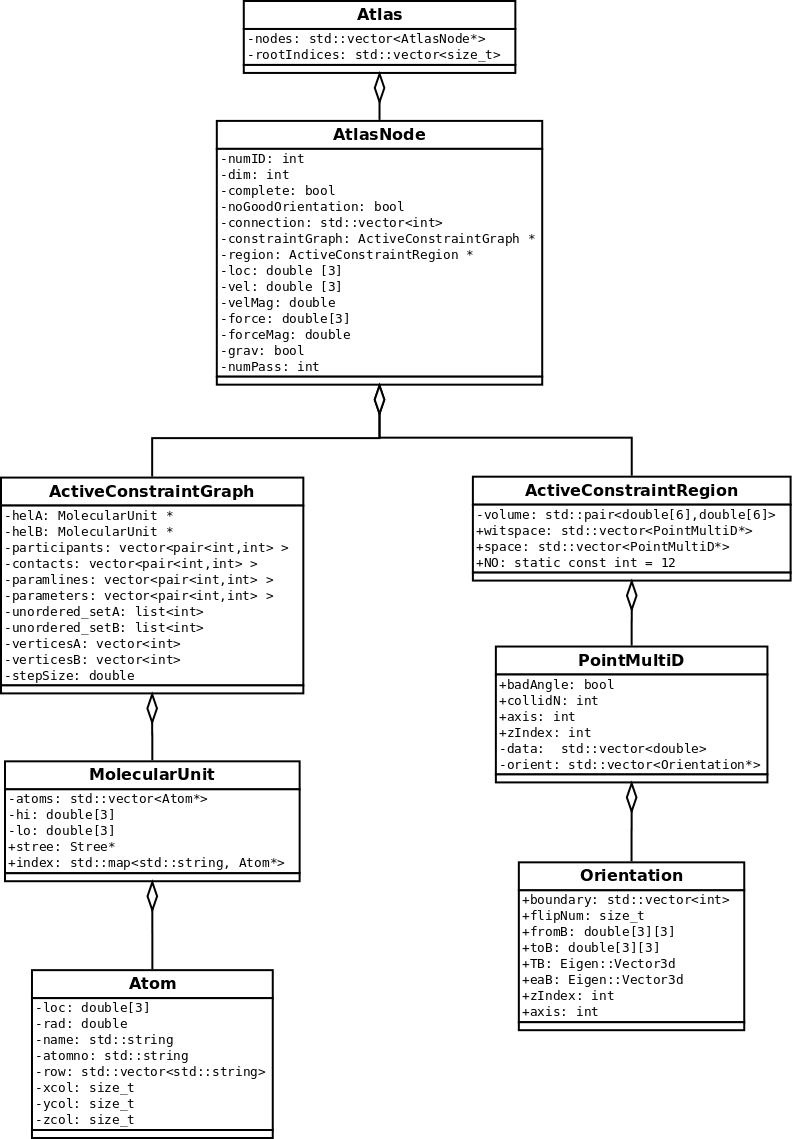
\includegraphics[scale=0.3] {fig/EASAL_UML.png}
\caption{EASAL UML Diagram}
\label{UML}
\end{figure}


\figref{UML} gives an overview of the structure of the major classes of EASAL.
Each of these classes are explained in the subsections below.

\subsubsection{AtlasBuilder} 

The AtlasBuilder class populates the ActiveConstraintRegion for each
activeConstraintGraph by sampling inside the boundaries of its ConvexChart. 
It creates and explores only regions that contain at least one Cartesian
realization. 

\begin{algorithm} [htbp]
 \SetKwInOut{Input}{input}\SetKwInOut{Output}{output}

 {\bf sampleAtlasNode}\\
 \Input{atlasNode: node}
 \Output{Complete sampling of the atlasNode and all its children}
 \BlankLine
 \LinesNumbered
	$H$ = node.activeConstraints\\
	$G_H$ = node.activeConstraintGraph\\
	\If{ $G_H$ is minimally rigid}
		{stop;	}
	$F$ = complete3Tree($G_H$)\\
	
	$C$ = computeConvexChart($G_H$, $F$)\\

	\For{ each cayleyPoint $p$ within convexChart $C$ }
	{
		$R$ = computeRealizations($p$)\\

		\For{ each realization $r$ in $R$}
		{
			\If{!aPosterioriConstraintViolated($r$)}
			{
				\If{ isBoundaryPoint($r$) \&\& hasNewActiveConstraint($r$, $G_H$) }
				{
					$e$ = newActiveConstraint($r$, $G_H$);\\
					$G'$ := $G_H \cup \{e\}$ ;\\
					\If{ $G'$ is not already present in the current atlas}
					{
						childNode = new atlasNode($G'$)\\
						sampleAtlasNode(childNode);\\
					} \Else{
						childNode = findNode($G'$);
					}
					node.setChildNode(childNode);
				} 
			}
		}
	}

	\caption{High level EASAL pseudocode}
\label{alg:sampleAtlasNode}
\end{algorithm}


\noindent \textbf{Major Attributes:} 
\begin{itemize}
		\item  \textbf{rootGraphs}: The set of all possible 4D or 5D
				ActiveConstraintGraphs of the root nodes
				generated before sampling.
		\item  \textbf{atlas}: An atlas object that is populated by the
				AtlasBuilder by sampling. This object is shared between front-end and
				back-end of the algorithm.
\end{itemize}

\noindent \textbf{Major Methods:}
\begin{itemize}
		\item  \textbf{startAtlasBuilding()}: For each of the generated root graph, 
				creates an atlasNode labeled with a contact graph $G_F$ where $F$ is the
				set of contacts. Then calls the recursive sampleTheNode method 
				for each of the root atlas nodes.
		\item  \textbf{sampleTheNode(atlasNode)}: The exploration of the atlas
				is done by the recursive \textbf{sampleAtlasNode} algorithm (see Algorithm 
				\ref{alg:sampleAtlasNode})
				using one of the generated atlas root nodes as input. This
				algorithm is implemented by the sampleTheNode method. Using
				depth first search this algorithm samples the atlas node and
				all its descendants. 
				
				\textbf{Base case of recursion:} If active constraint graph $G_H$ of the 
				node is minimally rigid i.e., the active constraint region is 
				0-dimensional, we have no more sampling to do, return.
				
				\textbf{The recursion step:} If $G_H$ is not minimally rigid, we use the
				\textbf{complete3Tree} algorithm to find find a set of parameters $F$ so 
				as to form a maximal 3-tree to leverage the convex parametrization theory~
				\cite{SiGa:2010}. This also ensures that $H \cup F$ is minimally rigid and 
				easily realizable. 
				
				The method computeConvexChart shown in the pseudocode finds the convex 
				chart for the parameters $F$ is done by the ConvexChart class explained 
				later. Method ComputeRealizations computes the realization for a 
				Cayley point and is done by the findRealizations method in the software. 
				The aPosterioriConstraintViolated method which checks for angle and steric 
				violations is implemented in the ConstraintCheck class explained later.
				Next we make a call to the findBoundary to detect boundaries and
				newly active constraints.
				

		\item  \textbf{determineStepSizeDynamically()}: Finds out the step size $s$
				given $T$, the total number of samples. Each 5D atlas node has its
				own $s$ computed by using the volume of the Cayley parameter space of the
				node over total number of samples per node. The volume of the
				Cayley parameter space of the node is approximately computed by
				exhaustive sampling within the exact chart without considering
				any constraints. The number of samples per node roughly can be
				computed by $T$ over total number of root(starter) atlas
				nodes, $m$. The number of samples in child nodes are negligible
				since the volume of regions in low dimensional nodes are
				negligible compared to the regions of high dimensional nodes.
		
		\item  \textbf{findBoundary()}: Boundary detection ensures that sampling 
				stays in the feasible region and minimizes discarded samples. 
				The findBoundary method which detects boundary points, checks 
				for newly formed active constraints and makes function calls
				which in turn call sampleTheNode for a child region.
		
\end{itemize}

\subsubsection{Atlas} 
The `Atlas' class stores the directed acyclic graph that represents the relationship between active constraint regions.

\noindent \textbf{Major Attributes:}
\begin{itemize}
		\item \textbf{nodes}: A vector of all AtlasNodes. 
		\item \textbf{rootIndices}: The indices of all the root nodes in the atlas.
\end{itemize}

\noindent \textbf{Major Methods:}
\begin{itemize}
		\item \textbf{search(node)}: Uses depth first search on the atlas to check
				whether the node exists in the atlas or not. It is used to avoid
				repeated sampling of the same region. The time complexity of
				the search is $O((\text{depth of the tree})) = O(6(k-1)) $ which in our 
				case is $O(1)$ since we fix $k$ to be 2.
\end{itemize}


\subsubsection{AtlasNode} 
AtlasNodes make up the Atlas. Each AtlasNode represents an active constraint region
reperesented by an ActiveConstraintGraph.

\noindent \textbf{Major Attributes:}
\begin{itemize}
		\item \textbf{acg}: The active constraint graph corresponding to the node.
		\item \textbf{region}: The set of Cayley points in the active region.
		\item \textbf{connection}: The id of the nodes in the atlas that
				represent the boundary of this node's region.
\end{itemize}

\subsubsection{ActiveConstraintGraph} 
The ActiveConstraintGraph class is used to store the set of active constraints.

\noindent \textbf{Major Attributes:} 
\begin{itemize}
		\item  \textbf{activeConstraints}: The set of point index pairs that represent 
				contacts.
		\item  \textbf{verticesA}: Participating points from first point set.
		\item  \textbf{verticesB}: Participating points from second point set.
		\item  \textbf{parameters}: A vector of point index pairs that represent parameters.
\end{itemize}

\noindent \textbf{Major Methods:}
\begin{itemize}
		\item  \textbf{completeTo3by3Graph()}: Adds points to make sure there
				are at least 3 points from each point set so that the graph is
				realizable. While choosing additional points, it has 2 options,
				choosing the points closest to each other or the points that lead
				to a user specified angle.
\end{itemize}


\subsubsection{ActiveConstraintRegion} 
The ActiveConstraintRegion class contains the set of feasible Cayley points generated
by sampling.

\noindent \textbf{Major Attributes:} 
\begin{itemize}
		\item  \textbf{space}: The set of feasible Cayley points.
		\item  \textbf{witspace}: The set of feasible witness Cayley points
				obtained from an ancestor node.
\end{itemize}

\noindent \textbf{Major Methods:}
\begin{itemize}
		\item  \textbf{convertSpace(activeConstraintRegion)}: Re-parametrizes
				a region using an input region’s parameters. This method
				converts each Cayley point in the input activeConstraintRegion
				to the Cayley point parametrized by the input region's
				parametrization.
\end{itemize}


\subsubsection{CayleyPoint} 
The CayleyPoint class represents a multi-dimensional point in the Cayley parameter space
and stores the corresponding Cartesian space orientations of the point set.

\noindent \textbf{Major Attributes:}
\begin{itemize}
		\item  \textbf{data}: Values of the Cayley parameters (non-edge
				lengths). \item  \textbf{orients}: The set of Cartesian space
				Orientations of the point set that were computed by
				realizing the active constraint graph with the given length of
				the edges and non-edges.
\end{itemize}

\subsubsection{Orientation} 
The Orientation class is the Euclidean transformation of point set. The
Orientation class stores only the information necessary to compute the
transformation matrix that will yield a Cartesian realization for the entire
point set.

\noindent \textbf{Major Attributes:} 
\begin{itemize}
		\item  \textbf{FromB}: Cartesian coordinates of three points from the
				first point set before the transformation.
		\item  \textbf{ToB}: Cartesian coordinates of three points from the
				second point set after the transformation.
		\item  \textbf{connections}: The set of node indices that this
				orientation belongs to. An orientation be on the
				boundary of multiple regions.
\end{itemize}


\subsubsection{CayleyParameterization} 
The CayleyParameterization class chooses non-edges in an ActiveConstraintGraph
that convert the graph into complete 3-tree. Those non-edges are called the
parameters. The complexity of the sampling algorithm varies based on the
choice of non-edges and the order in which they are fixed.

\noindent \textbf{Major Attributes:} 
\begin{itemize}
		\item  \textbf{partial3tree}: A boolean variable indicating whether
				an ActiveConstraintGraph is partial 3-tree or not.
		\item  \textbf{parameters}: The set of points pairs that represent
				non-edges. 
		\item  \textbf{tetrahedra}: The ordered tetrahedron set that helps in 
				defining the order of parameters that is required
				during the sampling procedure. This data is later passed to
				ConvexChart and CartesianRealizer to help in their computations. 
		\item  \textbf{updateList}: Adjacency map containing the dependency of
				parameters. It provides the set of parameters whose range will
				be updated when one of the parameters is fixed.
		\item  \textbf{boundaryComputationWay}: Inequalities that express the
				range of a parameter can be classified into either a linear or
				non-linear class. This variable is the characterization of the
				parameter that tells what inequality is needed to compute
				the parameter range i.e., triangular or tetrahedral inequality. 
		\item  \textbf{complete3trees}: The set of complete 3 trees.
\end{itemize}

\noindent \textbf{Major Methods:}
\begin{itemize}
		\item  \textbf{defineParameters()}: The parameters of an active
				constraint graph are selected as maximal 3-realizable (3-tree)
				extensions by leveraging the convex parametrization theory.
				\cite{SiGa:2010}. It creates a look-up table containing all possible 
				complete 3-trees. We find a graph in the look-up
				table so that active constraint graph is a proper subset of either the 
				graph or one of its isomorphisms.
		\item  \textbf{parameterMinDeviation()}: An alternate way to pick
				the parameters for 5D regions is by ensuring that the range
				of each parameter is similar. The aim here is to sample more
				uniformly in the Cartesian space. 
		\item  \textbf{built3tree()}: The 3-tree formed by starting with a
				4-vertex complete graph and repeatedly adding vertices in
				such a way that each added vertex is edge-connected to the face
				of a tetrahedron. Store the tetrahedrons in the order they are
				created in the attribute \textbf{tetrahedra}.
\end{itemize}


\subsubsection{ConvexChart} 

The ConvexChart class is used to determine the \chart\ that parameterize the
regions i.e., it computes the range of parameters of ActiveConstraintGraph. An
exact convex chart yields feasible Cayley points for the current active
constraint region. The resulting Cayley configuration space is convex, before
collisions or other (e.g.\ angle) constraints are introduced. The range of
parameters are computed by triangle and tetrahedral inequalities.

\noindent \textbf{Major Attributes:} 
\begin{itemize}
		\item  \textbf{param\_lengthUpper}: The upper bound of the parameters' range 
		\item  \textbf{param\_lengthLower}: The lower bound of the parameters' range 
		\item  \textbf{param\_length}: current value of parameters
\end{itemize}

\noindent \textbf{Major Methods:}
\begin{itemize}
		\item  \textbf{initializeChart()}: Initalizes the boundaries of
				convex chart. Tighter bounds are given in \cite{ugandhar}. 
		\item  \textbf{computeRange(v1, v2)}: Computes the range of the
				parameter $v1-v2$ in order to eliminate sampling infeasible grid
				points. Range computation is required in every iteration for
				dependent parameters. 
		\item  \textbf{setRangeByTriangleInequality(v1, v2)}: Computes the
				range of the non-edge $v1-v2$ through triangular inequalities.
		\item  \textbf{setRangeByTetrahedralInequality(v1, v2, tetrahedron)}:
				Computes the range of the non-edge $v1-v2$ through tetrahedral
				inequality.
		\item  \textbf{stepGrid}: Sets parameter point to the next grid point
				within the computed range.
		\item  \textbf{stepNeighbour()}: Sets the parameter point to the neighbor
				grid point in all dimensions consecutively.
		\item  \textbf{stepGridBinary()}: Sets the parameter point to 
				somewhere between current point and neighbor grid point
				according to binary search procedure in findBoundary.
\end{itemize}


\subsubsection{CartesianRealizer} 
The CartesianRealizer class contains routines that
compute orientations that represent transformations of rigid helices
relative to each other. It computes Cartesian realization of an active 
constraint graph with the
parameter lengths taken from cayleyPoint and active constraint lengths for a
specific flip. 
\noindent \textbf{Major Attributes:} 
\begin{itemize}
		\item \textbf{positions}: Cartesian coordinates of vertices in
				ActiveConstraintGraph.
		\item \textbf{edge\_length}: Contains all fixed distances plus current
				distance values of non-edges of ActiveConstraintGraph.
\end{itemize}

\noindent \textbf{Major Methods:}
\begin{itemize}
		\item  \textbf{computeRealization(activeConstraintGraph, convexChart,
				flipno)}: Computes the Orientation by leveraging partial 3-tree
				techniques. activeConstraintGraph which is a complete 3-tree is
				built up from a base tethedra by adding, at each step, a new
				vertex edge-connected to the face of a tetrahedron.
		\item  \textbf{setBaseTetra(tetrahedron)}: Finds Cartesian
				coordinates of the vertices of tetrahedron by known edge
				lengths.
		\item  \textbf{locateVertex(vertex, face)}: Finds Cartesian
				coordinates of the vertex that is connected to the face of a
				tetrahedron.
\end{itemize}


\subsubsection{ConstraintCheck} 

The ConstraintCheck class is designed to check whether any non-active
constraints become active. Users have the option
to define a set of constraints of interest. In which case, the new constraint
activation check is done only for these. For an input Orientation,
ConstraintCheck first computes the Cartesian realization for the entire \helix\
then passes it to other subroutines to perform user specified constraint check such as
steric constraints or angle constraints.



\section{Part II: Optional GUI}
\label{part2}
\subsection{Dependencies and installation}
\label{sec:part2dependency}

\subsubsection{Dependencies}

This section discusses all the dependencies EASAL requires to run.

\begin{itemize} 
  \item Operating System: EASAL has been tested only on the following platforms:
  \begin{itemize}
	\item Ubuntu 12.04 or higher.
	\item Fedora 22 or higher.
	\item OS X 10.8 Mountain Lion.
\end{itemize}
EASAL  should work on any UNIX variant platform with little to no modifications.

\item We use Version 2.0 of the \emph{Eigen} library for linear algebra
computations. All necessary files pertaining to Eigen required by EASAL are
provided with the source code in the \emph{include} directory.  
   
\item For the GUI, we use OpenGL for visualization and the opensource
fox-toolkit Version 1.6 for windowing. See the installation section for
instructions on installing the necessary libraries.  
		  
\item We use \emph{simpleini} to read the settings from the settings.ini file.
All necessary files pertaining to simpleini are provided with the source code
in the include directory.

\item EASAL has been tested on the NVIDIA graphics card with the NVIDIA
proprietary driver (Version 331 or higher).

\item C++ compiler: EASAL requires one of the following compilers
\begin{itemize}
\item g++ Version 4.8 or higher.
\item clang++ Version 3.8 or higher.
\end{itemize}

\item EASAL uses the GNU Make utility to compile the source files. Make
Version 4.1 is required.
\end{itemize}

 
\subsubsection{Installation}
The software can be run either as a terminal application or with its associated
GUI.  The steps for running each of these versions has been explained here. You
will need to download and install some third party libraries and update the
makefile provided before you can successfully compile and run EASAL in the GUI
mode.  

\begin{itemize}
	\item Install GLUT 
	  \begin{itemize}
	  \item On Ubuntu 
	  	  \begin{itemize}
	  	  	\item sudo apt-get install freeglut3 freeglut3-dev binutils-gold
		  \end{itemize}
	 \item On Fedora
	 \begin{itemize}
	  	  \item sudo yum install freeglut-devel mesa-dri-drivers mesa-libGL 
\end{itemize}
	  \end{itemize}
     \item Install FOX-Toolkit (Version 1.6)
	   \begin{itemize}
		   \item On Ubuntu
		   \begin{itemize}
	   	   		\item sudo apt-get install libfox-1.6-0 libfox-1.6-dev
			\end{itemize}
		   \item On Fedora
		   	\begin{itemize}
		   		\item Download fox toolkit from \url{http://fox-toolkit.org/}
				\item Extract it using ``tar -xvzf libFox-1.6.X.tar.gz''
				\item Run configure using ``su ./configure''
				\item Install using ``su make install''
			\end{itemize}
		   \item on OS X
		   	\begin{itemize}
		   		\item brew install fox
		   	\end{itemize}

	   \end{itemize}
	 \item Install GNU Make
	   \begin{itemize}
	   	   \item On Ubuntu 
	   	   \begin{itemize}
			\item sudo apt-get install make
		   \end{itemize}	
		   \item On Fedora
		   \begin{itemize}
			\item yum install make
\end{itemize}
		   \end{itemize}
	 \item Run \emph{make} from the root/build directory.
	 \item To run EASAL run \emph{``bin/guiEASAL''} in a terminal from the root/build directory.
\end{itemize}% subsubsection  (end)





\subsection{Input/Output}
\label{sec:part2io}
\subsubsection{Input}
Input to EASAL is specified using the input window (see \figref{inputwindow}).
The main input features are the following:
\begin{itemize}
		\item \textbf{Two rigid point sets}: \emph{the data for molecule
		(A/B)} field is used to specify the rigid point sets. This accepts the
		data in the pdb format.  The user can either type in the location of
		the input point sets files or select it using the browse option. Once a
		file has been selected, the \emph{set data} option allows the user to edit
		the input data before starting sampling.
\item \textbf{The pairwise distance constraints (potential energy or enthalpy
		function)}: There are three types of constraints.

\item \textbf{Bonding threshold}: This is the range of distances between atoms
		where bond formation is feasible (i.e., the attractive forces dominate). 
		this is given as $\lambda*(r_i+r_j) 
		\pm \delta$ namely the Lennard-Jones well. 
		Here, $\lambda$ is specified by the lambda text field in
		the input window and $\delta$ is specified by the delta text box in the
		input window. $r_i$ and $r_j$ are the radii of the atoms participating
		in the reaction. When predefined interactions are specified, we use those
		for the bond formation and use the bonding threshold only for the hard-sphere
		potentials for the points not involved in the bond formation.

\item \textbf{Collision threshold:} This is the minimum distance between points
or atoms. This too is given as $\lambda*(r_i+r_j) \pm \delta$.
		
\item \textbf{Predefined Interactions}: Only when the constraints between these
pairs are active, are the corresponding configuration space regions explored. 
\end{itemize}

\subsubsection{Output}
The output is the \emph{atlas} (see \figref{fig:atlas}), i.e., a topologically stratified
set of sample feasible realizations or configurations of the two rigid point
sets. In EASAL the output is visualized by what we call the \emph{sweep view}. One
point set is  held fixed, while the other set is drawn many times to trace out
the set of all feasible realizations.


\begin{figure}
\begin{center}
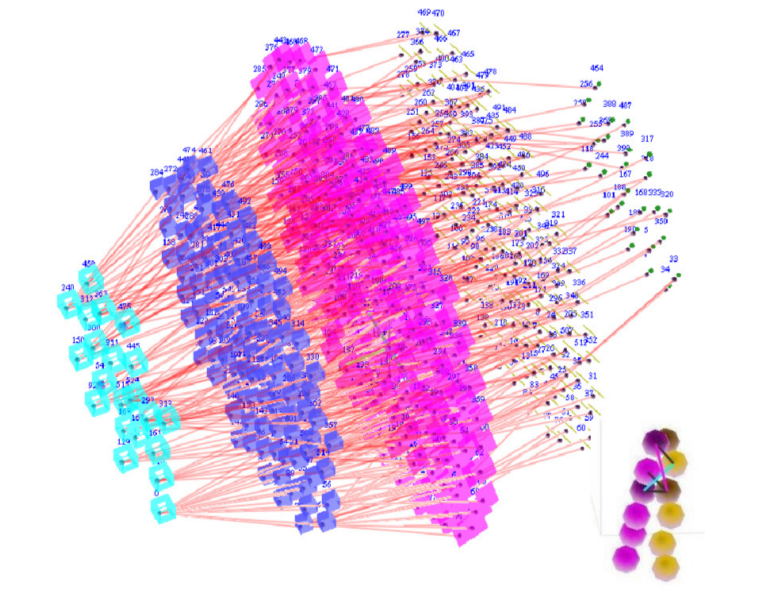
\includegraphics[width=.6\linewidth]{fig/Stratification.png}
\end{center}
\caption{Stratification of an assembly constraint system with atlas nodes of
dimension 4 (cyan), 3 (blue), 2 (purple), 1 (yellow), and 0 (green). Strata of
each dimension of the assembly constraint system visualized in the lower right
inset are shown as nodes of one color and shape in a directed acyclic graph.
Each node represents an active constraint region. Edges indicate boundary
relationships between a region and its parent region one dimension higher.}
\label{fig:atlas}
\end{figure}


\subsection{Software Functionalities}
\label{sec:part2functionalities}

This section introduces the main functionalities of EASAL.


\subsubsection{Stratification}
When EASAL first starts, the user is presented with the atlas view (see
\figref{atlasview}).  The atlas view shows the stratification of the
configuration space into regions of various dimensions, known as the active
constraint regions. The stratification is a directed acyclic graph where each
node represents an active constraint region and is associated with an active
constraint graph and edges represent boundary relationships.

\subsubsection{Active Constraint Graph}
When a node is clicked, EASAL automatically loads the active constraint graph
(see \figref{atlasview}) associated with that node in the bottom left corner.
This active constraint graph shows only the participating points from each set.
A solid edge between two points indicates a constraint and a dashed edge
indicates a parameter between two points belonging to different sets. It has to
be noted that the points in the same set already form a clique (not shown in
the graph).


\subsubsection{Finding Boundary Regions}
Clicking tree (see \figref{atlasview}) after selecting a particular node from
the atlas shows us all the boundary regions of that node. In terms of the
atlas, it shows the ancestors and descendants of that node . Edges indicate
boundary relationships between a region and its parent region one dimension
higher.. Note that the boundary regions are also shown in the Cayley space
view.



\subsubsection{Finding Paths Between Nodes With 6 Active constraints}
The atlas output by EASAL can be used to generate all the paths between any two
active constraint regions along with their energies. Once the atlas has been
generated, finding paths is extremely fast. The path topology of the assembly
configuration space is crucial for understanding assembly kinetics.

Of particular interest is finding paths between two lowest energy
configurations with 6 active constraints or 0D nodes of the atlas with
effectively rigid configurations. We are mainly interested in paths through
active constraint regions with 5 or 6 active constraints (which are one step
higher energy and have one fewer constraint). Such paths represent a continuous
one degree of freedom motion.

Whenever the user clicks on two nodes in succession, EASAL finds the path
between the two nodes, if it exists, and writes this path as a series of nodes
to the “paths.txt” file. Once the sampling has been completed, EASAL computes
the total number of paths of a particular length between every pair of vertices
and writes the entire matrix to the “path matrix.txt” file. The user can
specify lengths by setting the “path length” parameter in the settings.ini
file.


\subsubsection{Loading a Previously Generated Atlas}
\label{sec:loadAtlas}
EASAL gives the user the option to load a previously sampled atlas. To do this,
in the input window, enter the location of the data directory of the previously
generated atlas and click on the accept button. This gives a prompt with the
following options.


\begin{itemize}

\item Yes - Clicking on yes, loads the previously generated atlas.

\item No - Clicking on no, overwrites the atlas and writes fresh sampling
information to that locatin.

\item Cancel - Cancel allows the user to go back to the input window and change
the location of the data directory for this particular run.
\end{itemize}



\subsubsection{Sampling Options}
The user can at any point stop the current sampling mode and redirect the
sampling. The various options available are:
\begin{itemize}
\item \textbf{Stop Sampling}: Clicking this button stops the sampling of the
atlas and presents options to redirect the sampling.

\item \textbf{The Constraint Selection Dialogue Box}: This dialogue box (see
\figref {CSD}) allows the user to select a particular node from the atlas and
start sampling from that node. This feature gives users the flexibility to
explore regions of the graph that are more relevant to them. The user can
select a node by either specifying a node number or by specifying active
constraints between the point sets. The spheres with the indices denote the
atoms. A thick line between the atoms indicates a participating bond.  Here,
the first constraint is mandatory and hence does not have a \emph{connect}
check box next to it. The rest of the Active constraints are optional and the
user may choose up to six.
\begin{figure} 
\centering 
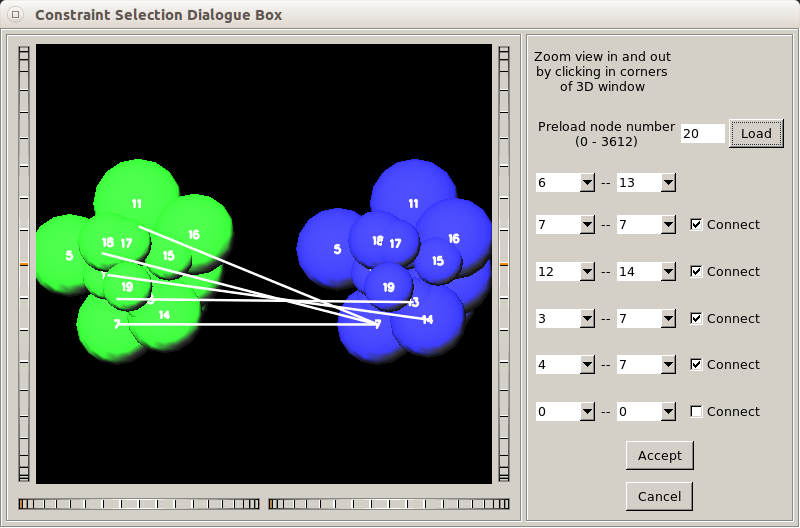
\includegraphics[scale=0.5]{fig/DumbbellSelection.png} 
\caption{Constraint Selection Dialogue} 
\label{CSD} 
\end{figure}

\item \textbf{CUR}: On clicking this, the sampling starts from the node that is
currently selected and ends when the tree in which the node is present is fully
sampled.

\item \textbf{Cleanup}: Clicking this completes sampling on all partially
sampled trees.

\item \textbf{A-S}: A-S stands for Auto-Solve. This button starts sampling in
the auto-solve mode. This is the default sampling mode. When starting afresh in
this mode, EASAL generates all possible 4D and 5D root nodes depending on the
user input. Then it proceeds to recursively sample all these nodes till the
atlas generation is complete. If there is a partially generated atlas, this
mode of sampling completes	 the unfinished trees and then proceeds to
sample all the other root nodes.

\item \textbf{BFS}: Clicking this button forces EASAL to explore the atlas in a
breadth first fashion which it otherwise does in a depth first fashion. In this
mode of sampling, EASAL starts from the node currently selected and samples its
subtree to completion.

\end{itemize}




\subsubsection{Dimension of the root node}
By default, the dimension of the root node of the atlas is 5, which means that
the root node has one bond and 5 parameters. The 4D root node option in the
advanced options (see \figref{advancedoptions}) allows the user to change this
and make the root node a 4D node. With a 4D root node, there are 2 bonds and 4
parameters in the root node.



\subsubsection{Convex Cayley Parametrization}
After selecting a node, the user can view its Cayley configuration space shown
in the Cayley space view (see \figref{Cayleyspaceview}). The Cayley space view
shows the active constraint region in the Cayley parametrized chart
representation for a particular node.




\subsubsection{Inspect Cayley Points}
The user can view the Cayley points in the Cayley Space View (see
\figref{Cayleyspaceview}). The Cayley points are shown on a 3D grid. For nodes
of dimension higher than 3D, one slider per extra dimension is given to view
the points in the $4^{th}$ and $5^{th}$ dimensions.  Categorization of Cayley
points: In the Cayley Space View (see \figref{Cayleyspaceview}), initially
green points are shown which correspond to all the realizable points in the
Cayley space. Clicking on the red square at the bottom shows the points that
have collision. Clicking the red square also shows two more options viz., cyan
and pink. The cyan points represent the points which have angle violations and
the pink points represent points which have distance violations. Clicking on
the blue square shows all the points sampled. The blue points represent
geometrically infeasible points.

\subsubsection{View Boundaries}
EASAL allows the user to inspect the points that form the boundary between a
region and its parent/child.  The boundaries option allows the user to inspect
the boundaries of the Cayley space. The user can step through each of the
boundaries using arrows provided.

\subsubsection{Step Size}
EASAL uses Cayley grid sampling to sample the Cayley space. The user can
specify this step size in the input window (see \figref{inputwindow}). Another
option available to the user is to choose the dynamic step size option in the
advanced window (see \figref{advancedoptions}). This tells EASAL to determine
the step size based on the volume of the space it is sampling. Once a space has
been sampled, there is always the option of refining the sampling.  This can be
done by selecting the refine sampling option in the atlas view whereupon EASAL
halves the step size and re-samples all the sampled spaces.

\subsubsection{Cartesian Realization}
The realization view (see \figref{realizationview}) in EASAL shows the
Cartesian realization of the Cayley points.

\subsubsection{View the sweep and flips of the Cartesian realization}
The sweep feature of a realization keeps one of the point sets units fixed and
draws all the possible orientations the other point set can take relative to
the first one (see \figref{realizationview}). The user can view the sweep. When
the sweep is being displayed, the user can use the arrow keys to view the
different flips.

\subsubsection{View realization along boundaries}
Clicking on the boundaries control allows the user to view the realizations
along the boundary region. The user can view it walk through the boundary
realizations using the arrows provided. Different colors are used to indicate
the realizations along different boundaries.

\subsubsection{View all realizations}
The user can use the video controls at the bottom (see
\figref{realizationview}) to display all the realizations of a region one after
the other. This differs from the sweep view in that sweep view shows all the
realizations at the same time.




\subsection{Sample Run}
\label{sec:run}
This section shows a sample run of EASAL. This sample run is illustrated in the 
latter part of the following video 
\url{http://www.cise.ufl.edu/~rprabhu/EASALvideo.mpg}.

\begin{itemize}

\item To run the software, run the following command from the top directory:
\emph{`bin/guiEASAL -settings $<$settings file name$>$'}.  Where $<$settings file
name$>$ is the path to the settings.ini file in which the input has been
specified. This loads preset inputs from the settings file, but can be modified
in the input window (discussed in the next step).


\begin{figure}
	\centering
	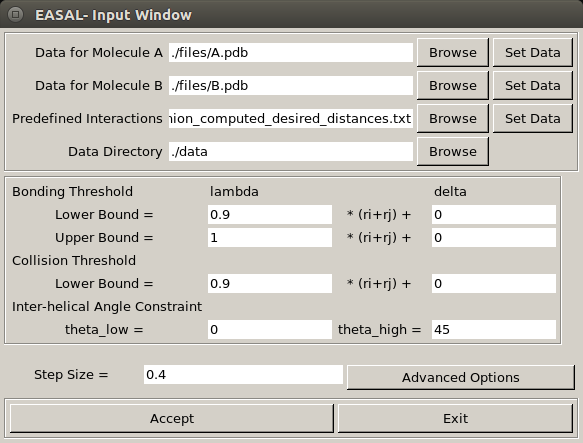
\includegraphics[scale=0.5] {fig/InputWindow.png}
	\caption{- In the input window, select the following either using the
	browse option or by entering the text in the text box provided\\
    - Data for Molecule A - files/A.pdb\\
    - Data for Molecule B - files/B.pdb\\
    - Distance Data - files/source\_files/union\ computed\ desired\ distances.txt\\
    - Data Directory - data/\\
    - Enter the values for Bonding Thresholds and step size .
}
	\label{inputwindow}
\end{figure}


\item The user can then click on the \emph{advanced options} button to set
advanced user inputs. This opens a new pop-up where the user can enter either
enter the data or choose to accept the default values.

\begin{figure}
\centering
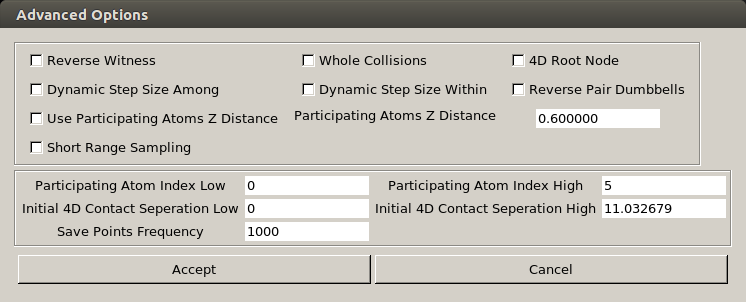
\includegraphics[scale=0.5] {fig/AdvancedOptions.png}
\caption{Advanced Options Window}
\label{advancedoptions}
\end{figure}

\item Click on \emph{accept} in the input window. This opens the Atlas View.

\begin{figure}
	\centering
	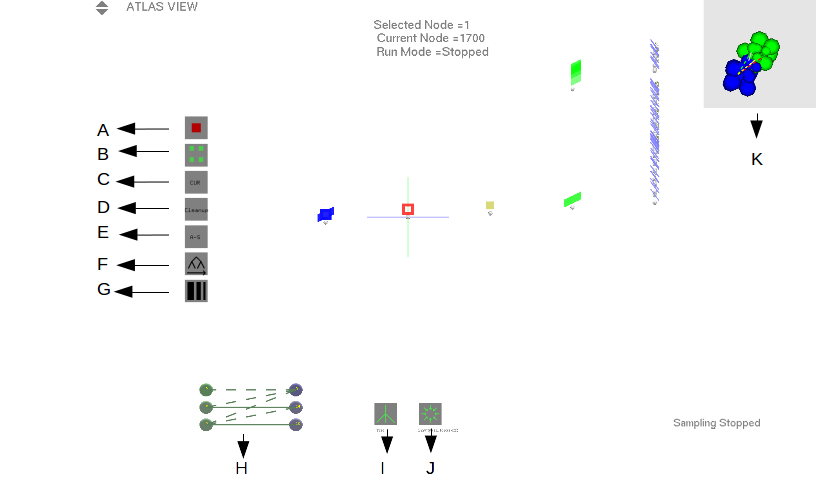
\includegraphics[scale=0.5] {fig/AtlasView.png}
	\caption{The Atlas View in EASAL . (A) Button to stop the sampling. (B) Button
to start the constraint selection dialogue box. (C) Button to continue sampling
the current tree. (D) Button to Clean Up Sampling. (E) Button to run EASAL in
the Auto-Solve mode. (F) Button to start exploring the Atlas in a breadth first
fashion. (G) Button to refine the sampling using a smaller step size. (H)
Active Constraint graph of the node selected. The spheres with the indices
denote the atoms. A thick line between the atoms indicates a bond and a dotted
line indicates a parameter. (I) Button to toggle Tree View. (J) Button to
toggle Gravity. (K) Cartesian realization of the current node.}
\label{atlasview}
\end{figure}

\item In the Atlas View, we initially see a root node at the center of a 3D
		grid. As and when more nodes are discovered, they are populated on the
		Atlas.

\item When the tree view is on, it shows only the ancestors and descendants of
		the node selected. When it is off, it shows the entire atlas. This can
		also be achieved by clicking the Tree control at the bottom.

\item In this view, the user can control how the sampling proceeds by using any
		of the controls on the left side of the atlas. The different controls
		available are (in the order they appear)
    - Stop Sampling.
    - Constraint Selection Dialogue Box.
    - Sample the Current Tree.
	- Sample all Incomplete Trees.
	- Auto-Solve.
    - BFS Sampling.
    - Refine Sampling.

\item Clicking on a particular node does the following - Loads the Active
		Constraint Graph at the bottom left corner.  - Loads the Cartesian
		realization for that node in the top right corner if the sampling for
		the node is complete.

\begin{figure}
	\centering
	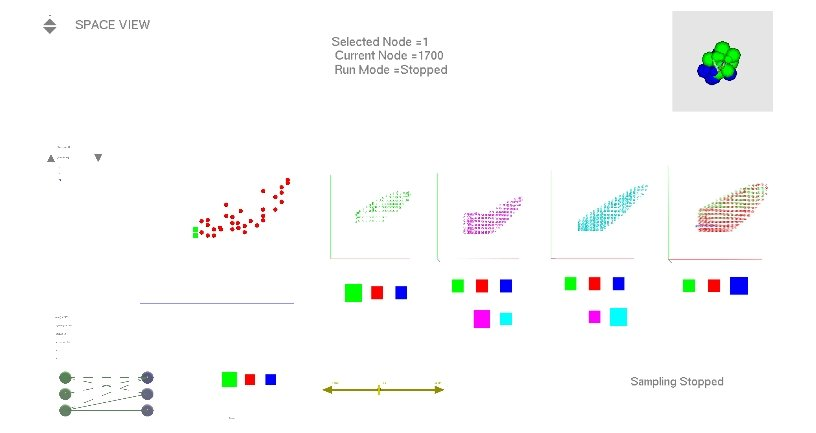
\includegraphics[scale=0.5] {fig/CayleySpaceView.jpg}
	\caption{Cayley Space View. The points outside the box show the boundary
points. The points in the box show the various Cayley points. From left to
right Good points, Collision points, points which violate the steric
constraints and all the points sampled.}
\label{Cayleyspaceview}
\end{figure}


\item Pressing the space bar after selecting a node takes the user to the
		Cayley space view of that node.

\item In the Cayley Space View, initially green points are shown which
		correspond to all the realizable points in the Cayley space.

\item Clicking on the Red square at the bottom, shows the points that have
		collision. Clicking the red also shows two more options viz, cyan and
		pink. The Cyan points represent the points which have angle collision
		and the pink points represent points which have distance collision.

\item Clicking on the Blue square shows all the points sampled including, the
		good, the collision and the unrealizable.

\item Clicking on the Boundaries shows the boundary points and the user can
		step through them along each dimension.

\begin{figure}
	\centering
	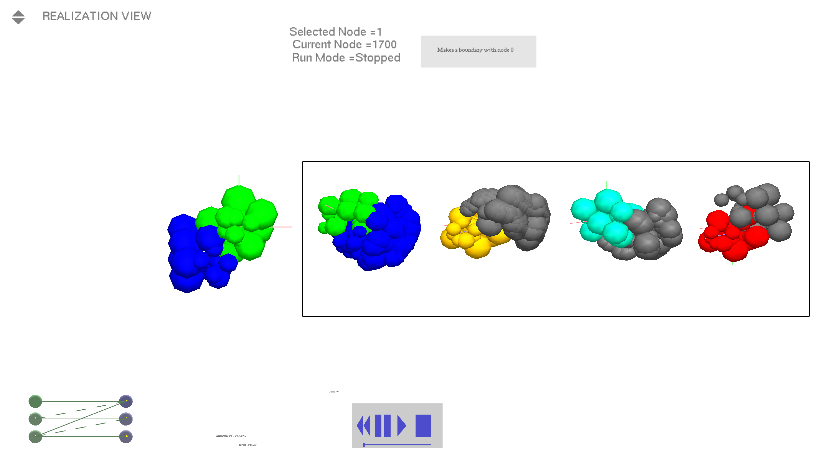
\includegraphics[scale=0.5] {fig/RealizationView.png}
	\caption{Realization View. The images in the box show the different
		realizations along different boundaries.}
		\label{realizationview}
\end{figure}

\item Pressing the space bar here takes the user to the \emph{realization view}.

\item Pressing \emph{v} on the keyboard generates the sweep view of the point set.

\item Once the sweep view is generated, the user can use the up and down arrow
		keys to view all the flips of the point set.

\item Clicking on boundaries shows the different realization along different
		boundaries.

\item Clicking on the video controls at the bottom and clicking the play button
		on it animates and shows all the possible realizations of the point set.
\end{itemize}






\bibliographystyle{plain}
\bibliography{easal}

\end{document}
